\chapter{Probabilistic approach}
\section{core idea}
we have two main points of views:
\begin{itemize}
    \item \textbf{traditional view}: we wanna to approximate a function $f:X\to X$
    \item \textbf{Probabilist view}: we wanna compute probablilities: $p: P( Y\mid  X)$
\end{itemize}
\subsection{Probs basics}
\subsubsection{Random variables}
A random variables $X$ represents an oyt come about which we're ncertain
\ex{Random variables}{
\begin{itemize}
    \item $X=$\texttt{true} if a randomly drawn stdent is male
    \item $X=$ first name of the student
    \item $X=$\texttt{true} if a randomly drawn stdent have the same birthday
\end{itemize}
}
 
Formal def:
\dfn{Probs variables}{
    the set $\Omega$ of the possible outcomes is called the sample space. It is said random variable a measurable function over $\Omega$:
    \begin{itemize}
        \item Discrete: $\Omega \to \{m,f\}$
        \item Continuos: $\Omega\to \mathbb{R}$
    \end{itemize}
}
 
\dfn{Probs def}{
    it is defined $P(X)$ is the fraction of times $X$ is true in repeated runs of the same experiment.
}

\nt{
    The definition requires that all samples 
}

Pay attention:
\wc{
    bad examples
}{
    Sample space, let $\Omega$ be a space made the possibile sum:
    \[
        \Omega = \{2,3,4,\dots, 12\}
    \]
    Problem: not all sums are equally likely! It should be:
    \[
        \begin{array}{c}
            P(sum = 2) = 1/11\\
            P(sum = 7) = 1/11
        \end{array}
    \]
    but in reality:
    \begin{itemize}
        \item Sum = 2: can only happen one way: $(1,1)$
        \item Sum = 7: can happen six ways:$(1,6), (2,5), (3,4), (4,3), (5,2), (6,1)$
    \end{itemize}

    so 
    \[
        P(sum = 2) \neq P(sum = 7)
    \]
}

A correct approach is 
\clm{correct approach}{}{
    Be $\Omega = {(1,1), (1,2), (1,3), ..., (6,5), (6,6)}$, where $|\Omega|=36 $outcomes

    each pair has equally probability = $\frac{1}{36}$
    
    Now here is a correctly computing:
    \[
        \begin{array}{c}
            P(sum = 2) = \frac{|{(1,1)}|}{36} = \frac{1}{36}\\
            P(sum = 7) = \frac{|{(1,6), (2,5), (3,4), (4,3), (5,2), (6,1)}|}{36} = \frac{6}{36}
        \end{array}
    \]
}

\subsubsection{The Axioms of Probability Theory}
These are the fundamental rules that make probability a "reasonable theory of uncertainty":

\ax{Axioms of probability theory}{
    \begin{align}
        &\text{(1) Non-negativity: } && 0 \leq P(A) \leq 1 \quad \text{for all events } A. \\
        &\text{(2) Normalization: } && P(\Omega) = 1. \\
        &\text{(3) Countable additivity: } && 
        \text{If } A_1, A_2, \dots \text{ are disjoint, then } 
        P\!\left(\bigcup_{i=1}^\infty A_i\right) = \sum_{i=1}^\infty P(A_i).
    \end{align}
}

Then:

\cor{consequences of the axioms}{
\begin{itemize}
    \item Monotonicity: If $A \subseteq B$, then $P(A) \le P(B)$
    \item Union rule (for two events): $P(A \cup B) = P(A) + P(B) - P(A \cap B)$
    \item $P(True) = 1$
    \item $P(False) = 0$
\end{itemize}
}

\begin{center}
    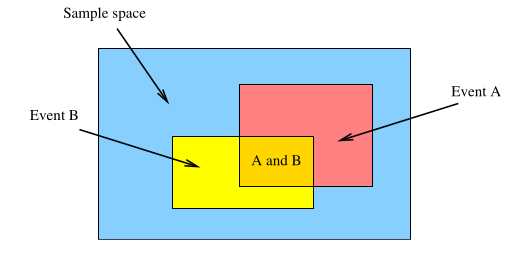
\includegraphics[width=5cm]{probs_ax.png}
\end{center}

\subsubsection{Derivied theorems}
\cor{Complement Rule
}{
    \[
        P(\lnot A) = 1- P(A)
    \]
}
\pf{Dm}{
\[
P(A \cup \neg A) = P(A) + P(\neg A) - P(A \cap \neg A)
\]

But: 
\[
P(A \cup \neg A) = P(\text{True}) = 1
\quad \text{and} \quad
P(A \cap \neg A) = P(\text{False}) = 0
\]

Therefore:
\[
1 = P(A) + P(\neg A) - 0
\quad \implies \quad
P(\neg A) = 1 - P(A) \qed
\]

}

\cor{Partition Rule}{
    \[
        P(A) = P(A \cap B) + P(A \cap \neg B)
    \]
}
\pf{Proof}{
    \[
\begin{aligned}
A &= A \cap (B \cup \neg B) &\text{[since $B \cup \neg B$ is always True]}\\
  &= (A \cap B) \cup (A \cap \neg B) &\text{[distributive law]}
\end{aligned}
\]

Hence,
\[
\begin{aligned}
P(A) &= P((A \cap B) \cup (A \cap \neg B)) \\
     &= P(A \cap B) + P(A \cap \neg B) - P((A \cap B) \cap (A \cap \neg B)) \\
     &= P(A \cap B) + P(A \cap \neg B) - P(\text{False}) \\
     &= P(A \cap B) + P(A \cap \neg B)
\end{aligned}
\]

}
\subsubsection{Multivalued Discrete Random Variables}
\dfn{
    k-value Discrete Random Variables
}{
    A random variable $A$ is \textit{$k$-valued discrete} if it takes exactly one value from 
    \[
    \{\nu_1, \nu_2, \dots, \nu_k\}.
    \]
}

\mprop{Key proprieties}{
    \begin{enumerate}
    \item \textbf{Mutual exclusivity:} For $i \neq j$,
    \[
        P(A = \nu_i \cap A = \nu_j) = 0
    \]

    \item \textbf{Exhaustiveness:}
    \[
        P(A = \nu_1 \cup A = \nu_2 \cup \dots \cup A = \nu_k) = 1
    \]
\end{enumerate}

}

\subsubsection{Conditional Probability}
\dfn{Conditional probs}{
    The Conditional probs of the event $A$ \textit{given} the event $B$ is defined as the quantity
    \begin{center}
        \begin{math}
            P(A\mid B) = \frac{P(A\cap B)}{P(B)}            
        \end{math}
    \end{center}
}

\cor{Cahin roule}{
    \[
        P(A\cap B) = P(B)P(A\mid  B)= P(A) P(B\mid A)
    \]
}
\subsubsection{Independent Events}
\dfn{Independent Events}{
    Events $A$ and $B$ are independent when:
    \begin{center}
        \begin{math}
            P(A\mid  B) = P(B)
        \end{math}
    \end{center}
}
(Meaning: B provides no information about A.)
\cor{consequences}{
    \begin{itemize}
        \item $P(A\cap b) = P(A)P(B)$ (from chail roule)
        \item $P(B|A) = P(B)$ (symmetry)
    \end{itemize}
}

\subsubsection{Bayes' Rule: The Heart of Probabilistic ML (ok chat... really?)}
\thm{Bayes's roule}{
    Now we have Bayes roule
    \begin{center}
        \begin{math}
            P(A\mid  B) = \frac{P(A)  P(B\mid A)}{P(B)}
        \end{math}
    \end{center}
}
\pf{Proof}{
    It's true by the chain roule that: $P(A \cap B) = P(B)  P(A\mid B)$. It's true also the reverse case $P(A \cap B) = P(B) · P(A\mid B)$.

    Since both expressions equal $P(A \mid B)$, they must equal each other:
    \[
        P(A)  P(B\mid A) = P(B)  P(A\mid B) 
    \]
    that it's equal to
    \[
        P(A\mid B) =\frac{[P(A)  P(B\mid A)]}{P(B)}
    \]
}
\ex{The trousers problem}{
    Setup:
    \begin{itemize}
        \item 60\% of students are boys, 40\% are girls
        \item girls wear in the same number skirt and trousers
        \item boys only wear trousers
    \end{itemize}
    If we see a student wearing trousers, what is the probability that is a girl?
}
\pf{Solution}{
    The probs a priori that a strudent is a girl is
    \[
        P(G) = \frac{2}{5}
    \]
    the probability that a student wears trousers is
    \[
        P(T) = \frac{1}{5} + \frac{3}{5} = \frac{4}{5}
    \]
    the probability that a student wear trousers, given that the student is a girl, is
    \[
        P(T\mid G) = 1/2
    \]
    So 
    \[
        P(G\mid T) =\frac{p(G)p(T\mid G)}{P(T)}=\frac{2/5\cdot 1/2}{4/5} = 1/4
    \]
}

\paragraph{Machine Learning Form}
\paragraph{Machine Learning Form}
For discrete $Y$ with values $\{y_1, y_2, \ldots, y_m\}$ and $X$ with values $\{x_1, x_2, \ldots, x_n\}$:
\[
P(Y = y_i \mid X = x_j) = \frac{P(Y = y_i) \cdot P(X = x_j \mid Y = y_i)}{P(X = x_j)}
\]

\textbf{Expanding the denominator:}
\begin{align*}
P(X = x_j) &= \sum_{i} P(X = x_j, Y = y_i) \quad \text{[sum over all $Y$ values]} \\
           &= \sum_{i} P(Y = y_i) \cdot P(X = x_j \mid Y = y_i) \quad \text{[chain rule]}
\end{align*}

\textbf{Complete Bayes' Rule:}
\[
P(Y = y_i \mid X = x_j) = \frac{P(Y = y_i) \cdot P(X = x_j \mid Y = y_i)}{\sum_{i} P(Y = y_i) \cdot P(X = x_j \mid Y = y_i)}
\]

\textbf{Terminology:}
\[
\underbrace{P(Y \mid X)}_{\text{posterior}} = \frac{\overbrace{P(X \mid Y)}^{\text{likelihood}} \cdot \overbrace{P(Y)}^{\text{prior}}}{\underbrace{P(X)}_{\text{marginal}}}
\]

\begin{itemize}
    \item \textbf{Posterior} $P(Y \mid X)$: What we want -- probability of $Y$ given observed $X$
    \item \textbf{Likelihood} $P(X \mid Y)$: How likely is $X$ if $Y$ is true?
    \item \textbf{Prior} $P(Y)$: What we believed before seeing $X$
    \item \textbf{Marginal} $P(X)$: Overall probability of observing $X$ (normalization constant)
\end{itemize}

\textbf{Alternative form:}
\[
\text{Posterior} = \frac{\text{Likelihood} \cdot \text{Prior}}{\text{Marginal Likelihood}}
\]
where:
\[
\text{Marginal} = \sum_{Y} P(X \mid Y) \cdot P(Y)
\]

The term ``marginal'' means we've \textbf{marginalized} (integrated/summed) over $Y$.

\section{The Joint Distribution}

\dfn{Joint Distribution}{
    Let $X_1, X_2,\dots, X_n$ be discrete random variables. The \textit{joint probability distribution} (or \textit{joint distribution}) of these variables is the function:
    \begin{center}
        \begin{math}
            P(X_1 = x_1, X_2 = x_2, \dots, X_n = x_n)
        \end{math}
    \end{center}

    which assigns to every possible combination of values \( (x_1, x_2, \dots, x_n) \) the probability that the random variables simultaneously take those values.

    Formally, for discrete variables, the joint distribution satisfies:
    \begin{itemize}
        \item \( 0 \leq P(x_1, x_2, \dots, x_n) \leq 1 \) for all \( (x_1, \dots, x_n) \)
        \item \( \sum_{x_1} \sum_{x_2} \cdots \sum_{x_n} P(x_1, x_2, \dots, x_n) = 1 \)
    \end{itemize}
}

Let's see an example
\ex{Joint distribution}{
    \begin{itemize}
        \item build a table with all possible combinations of values of random variables (features)
        \item compute the probability for any different combination of values
    \end{itemize}

    \begin{center}
        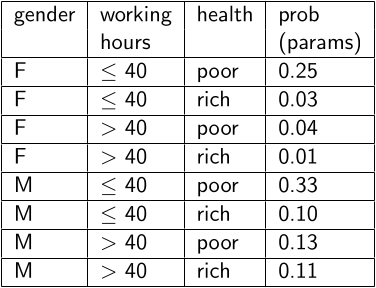
\includegraphics[width=6cm]{jd_img.png} % the table of the document
    \end{center}

    This table is the "Joint distribution"!

    Having that we may compute the probability of any event expressible as a logical combination of the features, with this formula
    \[
        P(E) = \sum_{row\in E} (row)
    \]
    in words for calculating an event we must add each row that is contained by the event. Let's provide an example (of an example)

        Let us compute the probability $P(M, poor)$
        \begin{center}
            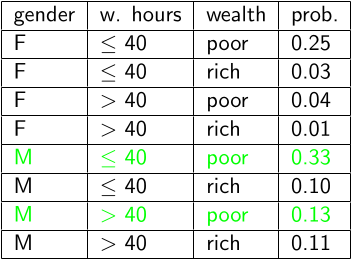
\includegraphics[width=6c]{jd_ex.png}
        \end{center}
    

    we have: $P(M, poor) = 0.33 + 0.13 = 0.46$
}

\subsection{Inference with the Joint distribution}
Here are with the inference:
\dfn{Contintional probability}{
    Let \( E_1 \) and \( E_2 \) be two events defined as logical conditions over subsets of the random variables (e.g., \( E_1: X_i = a, X_j = b \); \( E_2: Y = y \))

    Then, \textit{conditional probability} of \( E_1 \) given \( E_2 \) is:
    \[
        P(E_1 \mid E_2) = \frac{P(E_1 \land E_2)}{P(E_2)} = 
        \frac{\displaystyle\sum_{{row} \in (E_1 \land E_2)} P({row})}
        {\displaystyle\sum_{{row} \in (E_2)} P({row})}
    \]
}

for instance:
\ex{Conditional probability}{
    Let's compute $P(M|poor ) =\frac{P(M \land poor)}{P(poor)}$. We know that $P(M, poor ) = 0.46$. Let us compute $P(poor )$:
    \begin{center}
        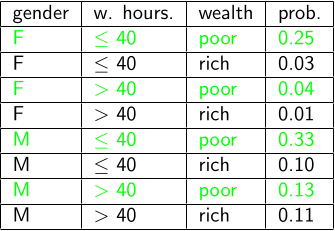
\includegraphics[width=6cm]{joint_inf.png}
    \end{center}
    Easy! $P(poor) = .75 \land P(M|poor) = 0.46/0.75 = 0.61$
}

\subsection{Complexity issues}
Let us build the joint table relative to
\[
    P(Y = wealth|X_1 = gender , X_2 = orelav.)
\]

\begin{center}
    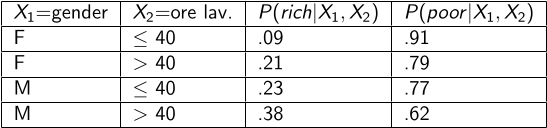
\includegraphics[width=6cm]{comp_issue.png}
\end{center}
To fill the table we need to compute $4=2^2$ parameters

If we have $n$ random variable $X = X_1 \times X_2 ,\dots, X_n$ where each $X_i$ is
boolean, we need to compute $2^n$ parameters. These parameters are \textit{probabilities}: to get reasonable value we would need a huge amount of data.

In particular the The Joint Distribution Requires \textit{Exponential parameters}
\ex{features and params}{
    \begin{itemize}
        \item With just 10 binary features, you need $2^{11}-1=2047$ parameters
        \item With 20 features: over 1 million parameters
        \item With 100 features: $2^{101}$ a number larger than the estimated atoms in the observable universe.
    \end{itemize}
}
This is computationally and statistically infeasible.
\subsubsection{USing Bayes}
for reducing complexity, we can rewrite the formula with the Bayes' rule:
\[
    P(Y=y_i\mid X=x_j) = \frac{P(Y=y_i)\cdot P(X = x_j\mid Y = y_i)}{\sum_i P(Y=y_i)\cdot P(X=x_j \mid Y=y_i)}
\]
generalising:
\[
    P(Y \mid X_1, X_2, \dots, X_n) = \frac{P(Y) \cdot P(X_1, X_2, \dots, X_n \mid Y)}{P(X_1, X_2, \dots, X_n)}
\]

But... there is a problem, it's required to know 
\[
    P(X_1, X_2, \dots, X_n \mid Y)
\]

that is the joint distribution of the features given $Y$, that requires, another time, $2^n$ params

\subsection{Naive Bayes}
For atteniung the complexity, it's possible assume an indipendencies conditional hypotesis, called "Naïve Bayes":
\[
    P(X_1,X_2,\dots,X_n|Y)=\prod_{i}P(X_i |Y)
\]
So given $Y$, $X_i$ and $X_j$ are independent from each other. In other therms:
\[
    P(X_i|X_j,Y)=P(X_i|Y)
\]
\nt{
    This means: onece we know $Y$, the feature $X_i \forall i$ are independents between each others
}
\ex{example 1}{
    A box contains two coins: a regular coin and a fake two-headed coin ($P(H) = 1$).Choose a coin at random, toss it twice and consider the following events:

    \begin{itemize}
        \item $A =$ First coin toss is H
        \item $B =$ Second coin toss is H
        \item $C =$ First coin is regular
    \end{itemize}
}
\ex{example 2}{
    For individuals, height and vocabulary are not independent, but they are if age is given.
}

\subsubsection{Giga formula with naive bayes}
\thm{Bayes rule}{
    \[
       P(Y = y_i \mid X_1, \dots, X_n) = \frac{P(Y = y_i) \cdot P(X_1, \dots, X_n \mid Y = y_i)}{P(X_1, \dots, X_n)}
    \]
}
\pf{Proof}{
    Left to mesco as exercice
}

\thm{Naïve Bayes}{
    \[
    P(Y = y_i \mid X_1, \dots, X_n) = \frac{P(Y = y_i) \cdot \prod_j P(X_j \mid Y = y_i)}{P(X_1, \dots, X_n)}
    \]
}
\pf{Proof}{
    Left to Bonzo as exercice
}

\thm{Classification of a new sample $x^{\text{new}} = \langle x_1, \dots, x_n \rangle$}{
    \label{thm:cne}
    Given a new instance represented by the feature vector $x^{\text{new}} = (x_1, x_2, \dots, x_n)$, 
    the predicted class is obtained as:
    \[
        Y^{\text{new}} = \arg\max_{y_i} \, P(Y = y_i) \cdot \prod_{j} P(X_j = x_j \mid Y = y_i)
    \]
}

\pf{Proof}{
    Left to Bastiality as an exercise.
}

\nt{
    Theorem~\ref{thm:cne} expresses the decision rule of the Naïve Bayes classifier.
    Given a new vector of features $x^{\text{new}} = (x_1, x_2, \dots, x_n)$, 
    we estimate the most probable class $y_i$ by maximizing the posterior probability 
    $P(Y = y_i \mid X_1 = x_1, \dots, X_n = x_n)$, 
    which—under the conditional independence assumption—reduces to the product of the prior $P(Y = y_i)$ 
    and the individual likelihoods $P(X_j = x_j \mid Y = y_i)$.
}

\section{Learning algorithm}
Given discrete Random Variables $X_i, Y$, there are two phases
\begin{itemize}
    \item \textbf{Training}: in this phases the maching learn from the data of training set, estimating two types of probs:
    \begin{itemize}
        \item \textbf{Prior}: (prob of the classes)
        \[
            \pi_k = P(Y = y_k)
        \]
        \item \textbf{Likelihoods}:(contained)
    \end{itemize}
\end{itemize}

